\chapter{Studi Literatur}

Pada bab ini, akan diisi oleh studi literatur, hal-hal yang berkaitan dengan topik persoalan tugas akhir akan dipaparkan dalam bab ini untuk memberikan informasi mengenai dasar teori dan studi yang dipakai. Bab ini diharapkan membantu pembaca untuk mengerti dalam membaca penelitian tugas akhir ini.

% TODO: banyak referensi yang kurang, klaim gaada referensinya
% TODO: only add relevent NLP task
\section{\textit{Natural Language Processing}}

Pemrosesan Bahasa Alami (PBA) atau dalam bahasa Inggris dikenal dengan \textit{Natural Language Processing} (NLP) merupakan cabang dari ilmu komputer, kecerdasan buatan, dan linguistik yang berfokus pada interaksi antara komputer dan bahasa manusia. NLP bertujuan untuk memungkinkan komputer tidak hanya memahami dan menafsirkan bahasa manusia, tetapi juga untuk menghasilkannya dengan cara yang bermakna dan efektif. Hal ini dijelaskan oleh \citeauthor{nlp} \parencite{nlp}, menyatakan pentingnya NLP dalam membangun jembatan komunikasi antara manusia dan mesin.

Dalam beberapa dekade terakhir, NLP telah mengalami kemajuan yang signifikan, memungkinkan komputer tidak hanya memahami bahasa manusia tetapi juga merespons dengan cara yang semakin kompleks dan kontekstual. Teknologi seperti mesin penerjemah, asisten virtual, dan sistem rekomendasi semuanya memanfaatkan prinsip-prinsip NLP untuk berfungsi.

Salah satu tantangan utama dalam NLP adalah keragaman dan kompleksitas bahasa manusia. Bahasa penuh dengan nuansa, ambiguitas, dan struktur yang dapat bervariasi tergantung pada konteks dan budaya. Untuk mengatasi tantangan ini, berbagai tugas NLP telah didefinisikan dan dikembangkan untuk memecah masalah pemahaman bahasa menjadi komponen yang lebih kecil dan lebih spesifik.

Beberapa tugas NLP yang umum antara lain \textit{Part of Speech} (POS) \textit{Tagging}, \textit{Named Entity Recognition} (NER), \textit{Dependency Parsing}, \textit{Sentiment Analysis}, dan \textit{Summarization}. Masing-masing tugas ini menargetkan aspek tertentu dari pemahaman bahasa dan memiliki aplikasi praktisnya sendiri dalam berbagai bidang, mulai dari analisis teks hingga pengembangan sistem percakapan otomatis.
\subsection{\textit{Part of Speech} (POS) \textit{Tagging}}

\textit{Part of Speech (POS) Tagging}, adalah proses mengkategorikan setiap kata dalam teks ke dalam kelas kata tertentu berdasarkan definisi dan konteksnya. Misalnya, kata "berlari" mungkin diberi tag sebagai verba, sementara "cepat" sebagai adjektiva. Tujuan dari POS tagging adalah untuk memahami fungsi kata dalam kalimat, yang penting dalam banyak aplikasi NLP lainnya.
\subsection{\textit{Named Entity Recognition} (NER)}

\textit{Named Entity Recognition} (NER) adalah tugas mengidentifikasi dan mengklasifikasikan nama entitas dalam teks ke dalam kategori seperti nama orang, organisasi, lokasi, dan lainnya. Misalnya, dalam kalimat "Barack Obama lahir di Hawaii", "Barack Obama"  dikenali sebagai nama orang dan "Hawaii" sebagai lokasi.

\subsection{\textit{Dependency Parsing}}

\textit{Dependency Parsing} adalah proses menentukan hubungan gramatikal antara kata-kata dalam kalimat. Ini menghasilkan struktur pohon di mana simpul adalah kata-kata dan tepi menunjukkan hubungan ketergantungan antara kata-kata tersebut. Misalnya, dalam kalimat "Ani memberi buku kepada Budi", kata "memberi" mungkin memiliki hubungan dengan "Ani" sebagai subjek dan "buku" sebagai objek langsung.
\subsection{\textit{Sentiment Analysis}}

\textit{Sentiment Analysis} adalah tugas mengidentifikasi dan mengekstrak opini atau perasaan dari teks. Tujuannya adalah untuk menentukan apakah pendapat yang dinyatakan dalam teks adalah positif, negatif, atau netral. Misalnya, "Saya suka film ini" memiliki sentimen positif, sementara "Saya membenci makanan di restoran itu" memiliki sentimen negatif.
\subsection{\textit{Summarization}}

\textit{Summarization} adalah proses mengurangi teks panjang menjadi versi yang lebih pendek yang tetap mempertahankan informasi penting. Ada dua pendekatan utama dalam ringkasan: ekstraktif, di mana kalimat atau frasa diambil langsung dari teks asli, dan abstraktif, di mana informasi diringkas dengan kata-kata baru. Misalnya, artikel berita panjang tentang kejadian tertentu dapat diringkas menjadi beberapa kalimat yang mencakup poin utama.

\section{\textit{Transformer}}

\textit{Transformer} telah mengubah lanskap pemrosesan bahasa alami (NLP) dengan cara yang signifikan. Dalam makalah mereka, penulis memperkenalkan konsep baru yang disebut mekanisme self-attention \parencite{transformers}. Mekanisme ini memungkinkan setiap kata dalam input untuk memfokuskan pada kata-kata lain dalam sekuens yang sama, memberikan model kemampuan untuk memahami konteks dengan lebih baik. Ini berbeda dari pendekatan sebelumnya yang biasanya mengandalkan informasi lokal atau posisi tetap dalam sekuens.

Salah satu keunggulan utama dari mekanisme self-attention adalah kemampuannya untuk menangani sekuens dengan panjang yang berbeda dan memahami hubungan antar kata tanpa mempertimbangkan jarak antara mereka. Ini memungkinkan Transformer untuk memahami ketergantungan jarak jauh dalam teks, sesuatu yang sulit dicapai oleh arsitektur sebelumnya seperti RNN dan LSTM.

Selain itu, Transformer dirancang untuk paralelisasi, yang memungkinkannya dilatih dengan cepat pada perangkat keras modern. Ini mempercepat penelitian dan pengembangan dalam NLP dan memungkinkan pelatihan model skala besar seperti BERT dan GPT yang sekarang mendominasi bidang ini.

Sejak diperkenalkannya Transformer, banyak variasi dan peningkatan telah dikembangkan. Namun, prinsip dasar self-attention dan paralelisasi yang diperkenalkan oleh Transformer tetap menjadi inti dari banyak inovasi dalam NLP kontemporer.

% TODO: add T5 and IndoT5
\section{\textit{Pre-Trained Model}}

\textit{Pre-trained model} merupakan model yang sudah dilatih terlebih dahulu pada \textit{dataset} yang berukuran besar sehingga model ini sudah mempunyai pemahaman yang mendasar pada tugas bahasa yang universal. \textit{Pre-trained model} dapat dilatih lebih lanjut terhadap suatu \textit{dataset} spesifik untuk menjalankan tugas bahasa yang spesifik juga. Salah satu \textit{pre-trained model} yang menjadi \textit{state-of-the-art} saat ini adalah BERT dan versi bahasa Indonesia-nya yaitu IndoBERT. 

\subsection{\textit{Bidirectional Encoder Representations from Transformers} \\ (BERT)}
\label{sec:bert}

BERT, yang merupakan singkatan dari \textit{Bidirectional Encoder Representations from Transformers}, adalah model \textit{encoder} pemrosesan bahasa alami yang diperkenalkan oleh Google pada tahun 2018 \parencite{bert}. BERT memanfaatkan arsitektur \textit{transformer}, yang telah dibahas sebelumnya, untuk memahami konteks kata dalam teks dengan cara yang lebih mendalam daripada pendekatan sebelumnya. BERT menggunakan pendekatan yang \textit{bidirectional}. BERT mampu memahami teks dari kiri ke kanan atau sebaliknya, BERT memahami konteks kata dengan mempertimbangkan informasi dari kedua arah. Sehingga, model ini memiliki kemampuan untuk pemahaman yang lebih kaya tentang makna dan nuansa dalam teks.

\begin{figure}[ht]
    \vspace{0.25cm}
    \centering
    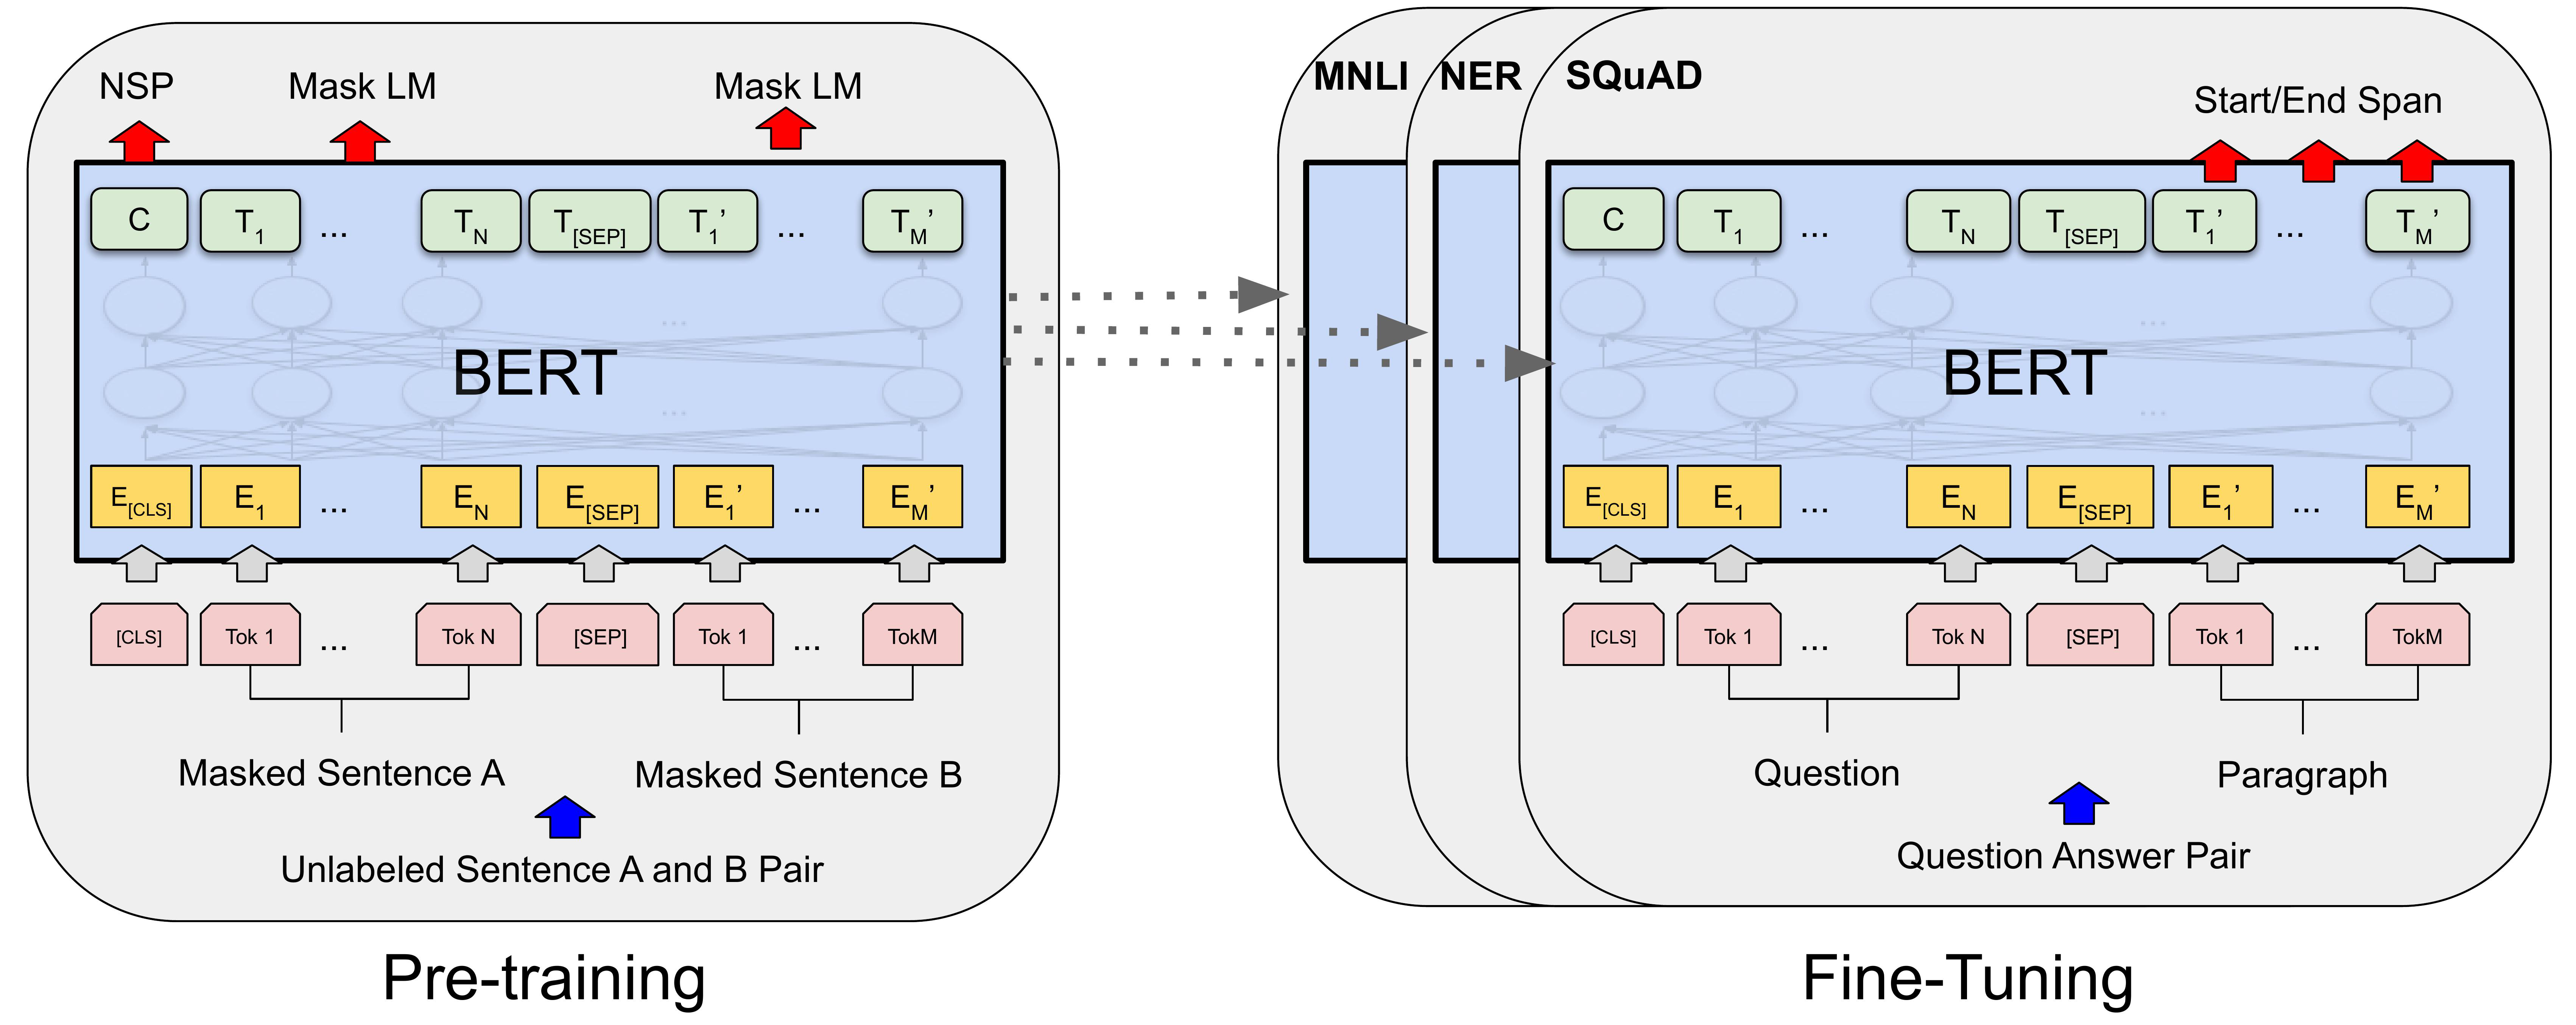
\includegraphics[width=\textwidth]{chapter-2/bert.jpg}
    \caption{Arsitektur BERT \parencite{bert}}
    \label{fig:bert}
\end{figure}

BERT merupakan \textit{pre-trained model} sehingga telah dilatih pada sejumlah besar teks. Data latih BERT diambil dari BooksCorpus dan Wikipedia bahasa Inggris \parencite{bert}. Ini memungkinkan BERT untuk mempunyai pengetahuan mendasar dalam tugas NLP. Ketika digunakan untuk tugas-tugas NLP spesifik, seperti klasifikasi teks atau pemahaman pertanyaan, BERT dapat disesuaikan dengan data tugas spesifik untuk meningkatkan kinerjanya. Seperti yang bisa dilihat pada gambar \ref{fig:bert}, BERT dilatih (\textit{pre-train}) dengan menggunakan dua tugas yaitu \textit{Masked LM} dan \textit{Next Sentence Prediction} (NSP). \textit{Masked LM} melakukan \textit{masking} pada sebagian token dan akan diprediksi oleh model BERT. Sedangkan, untuk NSP, model BERT akan menentukan mana kalimat berikutnya dari kalimat sebelumnya.

Terdapat versi bahasa Indonesia yaitu IndoBERT. IndoBERT merupakan model Transformer yang mirip dengan BERT, namun dilatih dengan bahasa Indonesia \parencite{indolem}. IndoBERT mempunyai konfigurasi yang sama dengan konfigurasi BERT, yaitu 12 \textit{layer} yang masing-masing mempunyai 768 \textit{hidden layer}, 12 \textit{attention head}, dan 3072 \textit{hidden layer} pada \textit{feed-forward layer}. IndoBERT dilatih dengan total 220 juta kata, yang didapatkan dari tiga sumber utama, yaitu Wikipedia Indonesia, sumber berita (Kompas, Tempo, dan Liputan6), dan Indonesian Web Corpus \parencite{indolem}. IndoBERT merupakan \textit{state-of-the-art} pada kakas evaluasi IndoLEM.

\subsection{\textit{Text-to-Text Transfer Transformers} (T5)}

\textit{Text-to-Text Transfer Transformers} atau biasa disebut sebagai T5 merupakan model \textit{encoder decoder} berbasis Transformer. Model ini menggunakan pendekatan \textit{text-to-text} seperti namanya, yang berarti menganggap setiap pemrosesan teks sebagai masukan dan mengeluarkannya sebagai teks juga \parencite{T5}. Dengan pendekatan ini, model T5 dapat digunakan secara langsung pada setiap tugas NLP.

\begin{figure}[ht]
    \vspace{0.25cm}
    \centering
    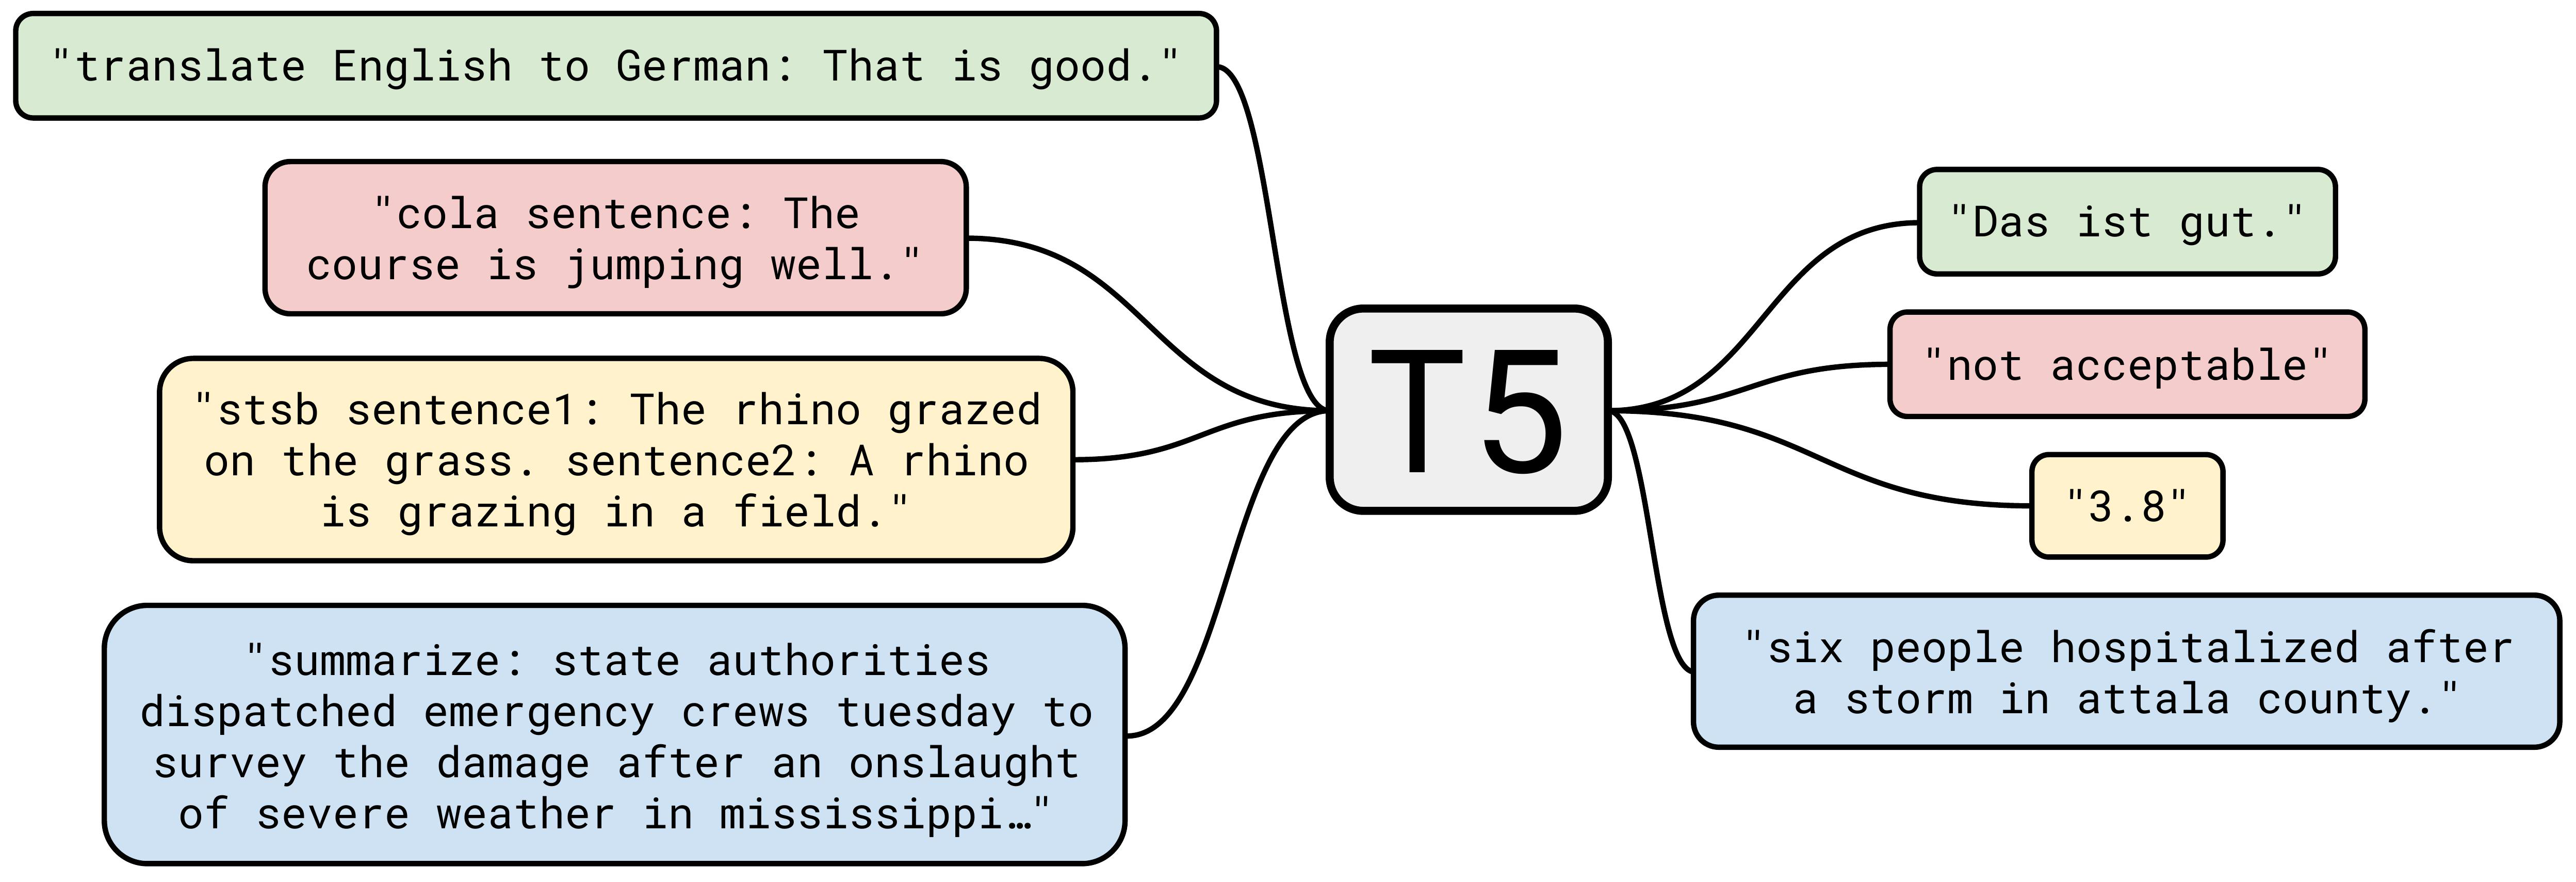
\includegraphics[width=\textwidth]{chapter-2/T5.jpg}
    \caption{\textit{Framework} dari T5 \parencite{T5}}
    \label{fig:T5}
\end{figure}

Pada gambar \ref{fig:T5}, yaitu \textit{framework} dari model T5, setiap tugas pada T5, termasuk \textit{translation, question answering}, dan \textit{classification}, semuanya akan dianggap sebagai masukan teks dan dilatih untuk menghasilkan teks lainnya lagi. T5 dilatih pada dataset \textit{Colossal Cleaned Crawled Corpus} (C4) yang merupakan koleksi dari web publik Common Crawl yang telah dibersihkan.

\begin{figure}[ht]
    \vspace{0.25cm}
    \centering
    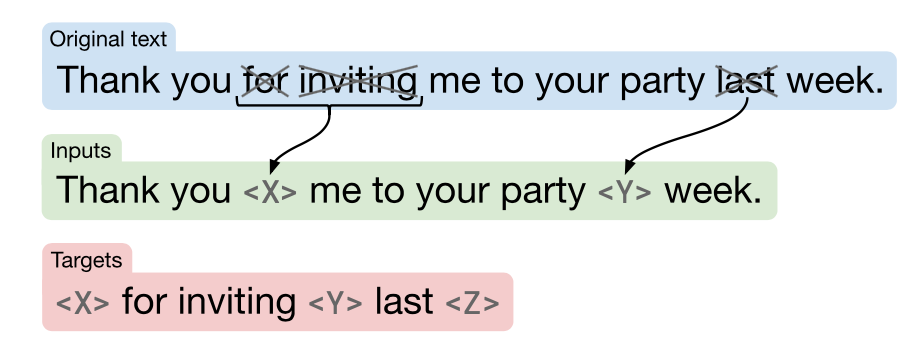
\includegraphics[width=\textwidth]{chapter-2/unsupervised_objective.png}
    \caption{\textit{Unsupervised objectives} dari T5 \parencite{T5}}
    \label{fig:unsupervised-T5}
\end{figure}

Model T5 didesain agar bagian \textit{encoder} dan \textit{decoder}-nya mirip dengan konfigurasi dari BERT \parencite{T5}. Kedua bagian tersebut terdiri dari 12 \textit{layer} yang mempunyai \textit{hidden layer, attention head}, serta \textit{feed-forward}. Mirip dengan MLLM pada BERT, model T5 dilatih \textit{pre-train} dengan menggunakan \textit{unsupervised objectives} yang bisa dilihat pada gambar \ref{fig:unsupervised-T5}. Beberapa kata yang dihilangkan secara konsekutif akan dianggap sebagai satu \textit{sentinel} token yang nantinya akan diprediksi sebagai target oleh T5.

Terdapat versi bahasa Indonesia dari T5, yaitu IndoT5. IndoT5 dilatih secara spesifik untuk bahasa Indonesia dengan menggunakan \textit{framework} pelatihan nanoT5 \parencite{indoT5}. \textit{Dataset} yang digunakan berasal dari CulturaX yang mengandung 23 juta dokumen berbahasa Indonesia. Model IndoT5 menjadi \textit{state-of-the-art} pada tugas \textit{summarization} pada kakas evaluasi IndoLEM.

\subsection{\textit{Bidirectional Encoder Representations from Transformers} \\ (BERT)}

BERT, yang merupakan singkatan dari \textit{Bidirectional Encoder Representations from Transformers}, adalah model pemrosesan bahasa alami yang diperkenalkan oleh Google pada tahun 2018 \parencite{bert}. BERT memanfaatkan arsitektur \textit{transformer}, yang telah dibahas sebelumnya, untuk memahami konteks kata dalam teks dengan cara yang lebih mendalam daripada pendekatan sebelumnya.

BERT menggunakan pendekatan yang \textit{bidirectional}. BERT mampu memahami teks dari kiri ke kanan atau sebaliknya, BERT memahami konteks kata dengan mempertimbangkan informasi dari kedua arah. Sehingga, model ini memiliki kemampuan untuk pemahaman yang lebih kaya tentang makna dan nuansa dalam teks.

\begin{figure}[ht]
    \centering
    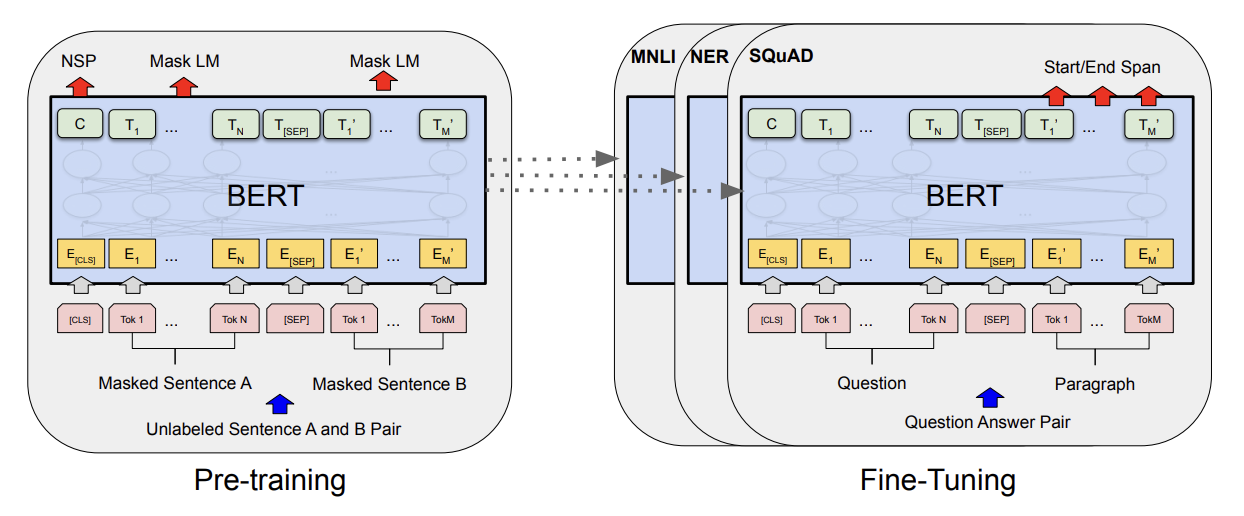
\includegraphics[width=0.8\textwidth]{chapter-2/bert.png}
    \caption{Arsitektur \textit{BERT} \parencite{bert}}
    \label{fig:bert}
\end{figure}

BERT merupakan \textit{pre-trained model} sehingga telah dilatih pada sejumlah besar teks. Data latih BERT diambil dari BooksCorpus dan Wikipedia bahasa Inggris. Ini memungkinan BERT untuk mempunyai pengetahuan mendasar dalam tugas NLP. Ketika digunakan untuk tugas-tugas NLP spesifik, seperti klasifikasi teks atau pemahaman pertanyaan, BERT dapat disesuaikan dengan data tugas spesifik untuk meningkatkan kinerjanya.

Model ini dikembangkan dengan dua konfigurasi, yaitu BASE dan LARGE. BERT dengan konfigurasi BASE memiliki 12 \textit{layer encoder} yang mempunyai 768 \textit{hidden layer} pada FFNN dan 12 \textit{attention heads}. Sedangkan, untuk konfigurasi BERT LARGE memiliki 24 \textit{layer encoder} yang mempunyai 1024 \textit{hidden layer} pada FFNN dan 16 \textit{attention heads}.
\subsection{IndoBERT}
\label{sec:indobet}

Meskipun terdapat lebih dari 200 juta pengguna bahasa Indonesia, bahasa tersebut kurang terwakili di NLP \parencite{indolem}. Sehingga, IndoBERT muncul untuk memperbaiki situasi ini. IndoBERT adalah adaptasi dari model BERT yang khusus dilatih untuk bahasa Indonesia. Mengingat keunikan dan kompleksitas bahasa Indonesia, memiliki model yang khusus dilatih untuk bahasa ini sangat penting untuk memastikan kinerja yang optimal pada tugas-tugas NLP yang berfokus pada bahasa Indonesia \parencite{indolem}.

\begin{figure}[ht]
    \centering
    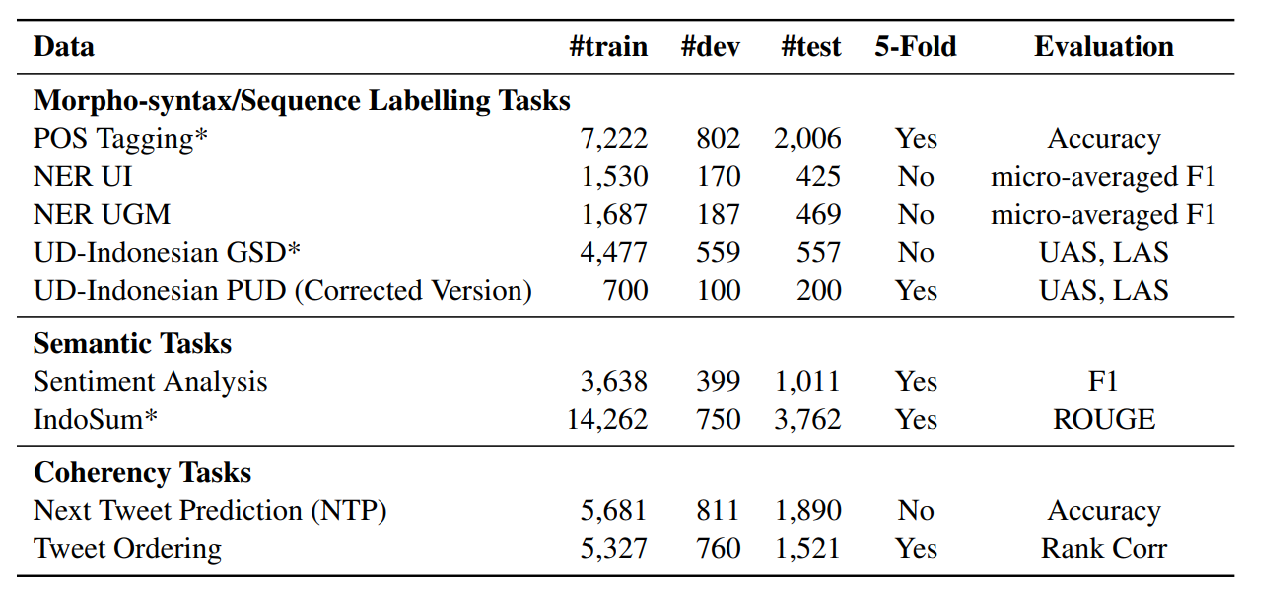
\includegraphics[width=0.8\textwidth]{chapter-2/indobert_dataset.png}
    \caption{\textit{Dataset} pada IndoBERT \parencite{indolem}}
    \label{fig:indobert_dataset}
\end{figure}

IndoBERT berbasis pada \textit{pre-trained model} BERT yang dilatih secara khusus pada \textit{dataset} berbahasa Indonesia, seperti yang bisa dilihat pada Gambar \ref{fig:indobert_dataset}. Tugas NLP yang dilatih pada IndoBERT dibagi menjadi tiga, yaitu \textit{sequence labelling}, \textit{semantic}, dan \textit{coherency}. Untuk \textit{sequence labelling} terdapat tiga tugas, yaitu \textit{part-of-speech} (POS) \textit{tagging}, \textit{named entity recognition} (NER), dan \textit{dependency parsing}. Lalu, untuk \textit{semantic} terdapat dua tugas, yaitu \textit{sentiment analysis} dan \textit{summarization}. Terakhir, untuk \textit{coherency} terdapat dua tugas, yaitu \textit{next tweet prediction} dan \textit{tweet ordering}.

\begin{figure}[ht]
    \centering
    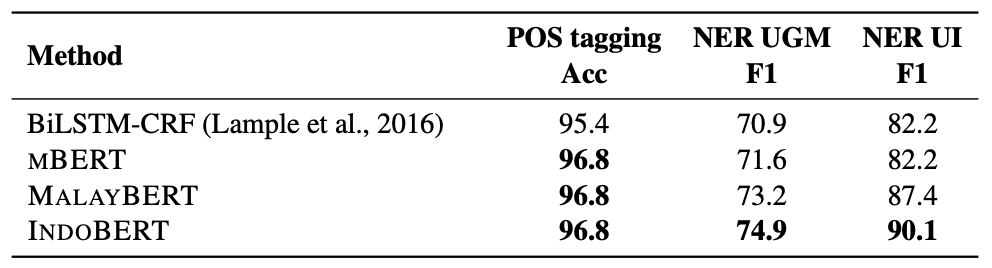
\includegraphics[width=0.8\textwidth]{chapter-2/indobert_pos.png}
    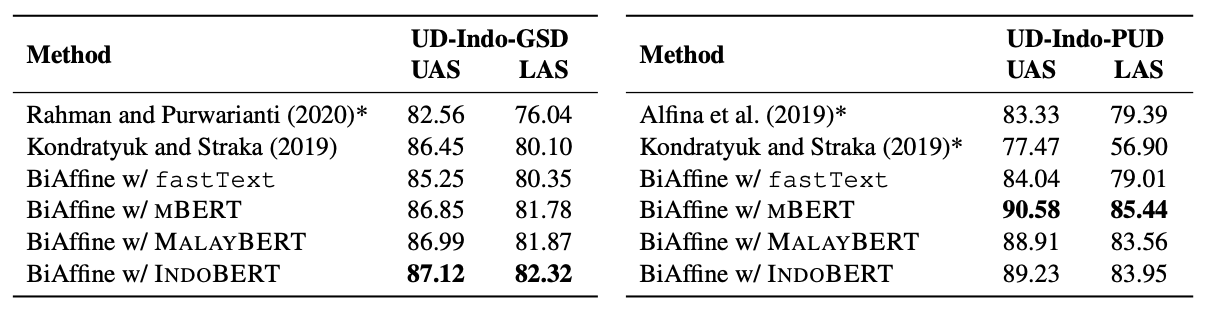
\includegraphics[width=0.8\textwidth]{chapter-2/indobert_dependency_parsing.png}
    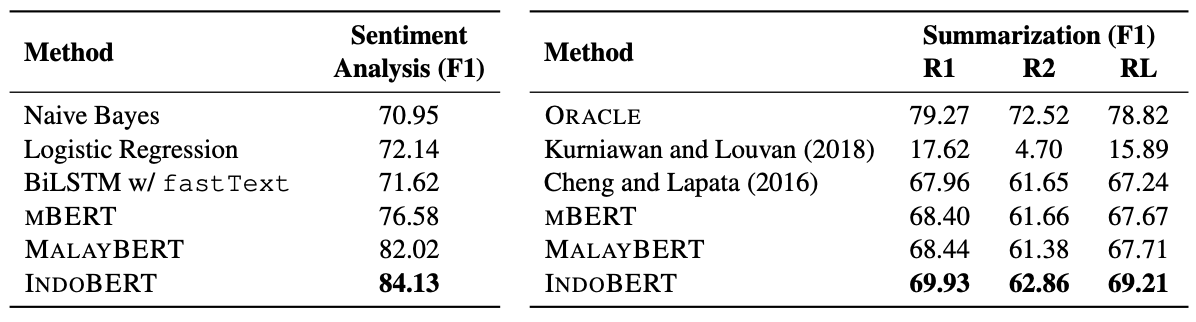
\includegraphics[width=0.8\textwidth]{chapter-2/indobert_semantic.png}
    \caption{Hasil Evaluasi IndoBERT \parencite{indolem}}
    \label{fig:indobert_evaluation}
\end{figure}

Untuk melakukan evaluasi terhadap model, dilakukan perbandingan dengan model lain. Pada penelitian ini, digunakan \textit{multilingual} BERT (mBERT) dan MalayBERT yang di-\textit{fine-tune} dengan bahasa Indonesia sebagai pembanding \parencite{indolem}. Hasilnya, IndoBERT kebanyakan unggul di setiap tugas. Selain dari tugas \textit{part-of-speech} (POS) \textit{tagging} dan \textit{next-tweet prediction} masih bisa dilakukan peningkatan \parencite{indolem}. Hasil evaluasi secara detail dapat dilihat pada Gambar \ref{fig:indobert_evaluation}.


\section{\textit{Transfer Learning}}

\textit{Transfer Learning} merupakan salah satu pendekatan kunci dalam pembelajaran mesin yang memanfaatkan model yang telah dilatih pada tugas tertentu sebagai dasar untuk melatih model pada tugas lain. Ide dasar di balik \textit{transfer learning} adalah bahwa, jika model telah mempelajari fitur-fitur tertentu dari satu tugas, fitur-fitur tersebut dapat digunakan sebagai informasi awal yang berguna untuk tugas lain.

Sebagai contoh, model yang telah dilatih untuk mengenali objek dalam gambar dapat memanfaatkan pengetahuannya tentang fitur visual, seperti tepi atau tekstur, saat dilatih untuk tugas pengenalan wajah. Meskipun tugas awal (mengenali objek) dan tugas kedua (pengenalan wajah) berbeda, ada sejumlah fitur visual yang relevan untuk kedua tugas tersebut.

Dalam konteks pemrosesan bahasa alami (NLP), \textit{transfer learning} sering digunakan untuk memanfaatkan \textit{Pre-Trained Model} (PLM) yang telah dilatih pada korpus teks besar untuk tugas-tugas spesifik seperti \textit{sentiment analysis} atau \textit{named entity recognition}. Dengan memulai dari model yang telah memiliki pemahaman dasar tentang struktur dan semantik bahasa, proses \textit{training} untuk tugas spesifik menjadi lebih cepat dan seringkali menghasilkan model yang lebih akurat dibandingkan dengan melatih model dari awal.

Keuntungan lain dari \textit{transfer learning} adalah efisiensi komputasi. Melatih model pembelajaran mesin dari awal, terutama model dengan banyak parameter, memerlukan sumber daya komputasi yang signifikan. Dengan menggunakan model yang telah dilatih sebagai titik awal, dapat menghemat waktu dan sumber daya komputasi, sambil mempertahankan atau bahkan meningkatkan kinerja model.


\subsection{\textit{Fine-Tuning}}

Salah satu metode yang sering digunakan untuk \textit{transfer-learning} adalah \textit{fine-tuning}. \textit{Pre-trained model} yang sebelumnya sudah dilatih pada data latih yang besar, dapat dilatih lebih lanjut untuk tugas NLP spesifik lainnya. Proses ini memerlukan \textit{dataset} tambahan, sehingga model dapat mendapatkan pengetahuan tambahan yang spesifik diperlukan terkait tugas NLP tersebut.

Proses \textit{fine-tuning} melanjutkan fase \textit{training} dengan \textit{dataset} tambahan yang diberikan kepada model. Sebelumnya, model mempunyai parameternya sendiri yang berasal dari proses \textit{pre-training}. \textit{Fine-tuning} membolehkan perubahan pada semua parameter model untuk menyesuaikan pada \textit{dataset} tambahan. Agar pengetahuan yang sebelumnya dimiliki oleh model tidak hilang ketika proses pengubahan parameter, \textit{learning rate} bernilai kecil bisa digunakan pada proses ini.

\textit{Fine-tuning} merupakan metode \textit{transfer learning} yang efisien ketika dilatih pada tugas spesifik dengan \textit{dataset} yang relatif kecil. Metode ini mengurangi kebutuhan akan sumber daya komputasi dan waktu yang besar, yang biasanya dibutuhkan untuk melakukan \textit{training} model dari awal.
\subsection{\textit{Low Rank Adaptation} (LoRA)}

Konsep dasar di balik LoRA adalah ide bahwa adaptasi model untuk tugas baru tidak selalu memerlukan perubahan besar pada seluruh parameter model. Sebaliknya, perubahan kecil pada representasi tertentu dapat menghasilkan peningkatan kinerja yang signifikan. Dengan fokus pada \textit{low rank adaptation}, LoRA mengubah hanya sebagian kecil dari bobot model, sementara sebagian besar bobot lainnya tetap tidak berubah. Ini berarti bahwa hanya "sebagian" dari informasi dalam model yang diperbarui, yang mengarah pada efisiensi komputasi yang meningkat \parencite{lora}.

\begin{figure}[ht]
    \centering
    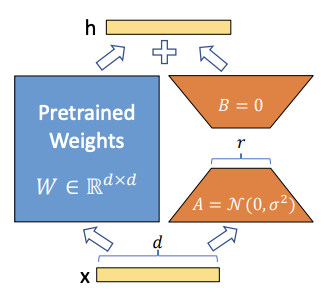
\includegraphics[width=0.8\textwidth]{chapter-2/lora.png}
    \caption{Arsitektur LoRA \parencite{lora}}
    \label{fig:lora}
\end{figure}

Salah satu kelebihan utama dari pendekatan ini adalah kemampuannya untuk mengurangi \textit{overhead} komputasi. Dalam praktiknya, ini berarti bahwa waktu \textit{training} dan sumber daya yang diperlukan untuk adaptasi model menjadi jauh lebih sedikit dibandingkan dengan metode lain yang mungkin melibatkan \textit{training} ulang model dari awal atau menambahkan sejumlah besar parameter tambahan. Arsitektur dari LoRA dapat dilihat pada Gambar \ref{fig:lora}

Pendekatan LoRA menjadi sangat relevan, terutama saat berhadapan dengan model-model berukuran besar. Model-model seperti ini memiliki jumlah parameter yang sangat besar, sehingga \textit{training} ulang atau menambahkan parameter tambahan bisa menjadi sangat mahal dari segi komputasi. Dengan LoRA, adaptasi model-model besar menjadi lebih praktis dan dapat dilakukan dengan efisiensi yang jauh lebih tinggi, tanpa mengorbankan kinerja.
Dengan demikian, LoRA menawarkan pendekatan yang menjanjikan untuk mengadaptasi \textit{pre-trained model} dengan cara yang lebih efisien.
\subsection{\textit{Prefix-Tuning}}

\textit{Prefix-Tuning} adalah teknik yang diperkenalkan untuk mengoptimalkan prompt kontinu dalam generasi teks. Berbeda dengan pendekatan tradisional yang melibatkan \textit{training} ulang seluruh model atau menambahkan parameter tambahan, \textit{Prefix-Tuning} fokus pada pengoptimalan sejumlah kecil parameter yang didefinisikan sebagai "prefix" dari sekuens input \parencite{prefix_tuning}. Dengan kata lain, alih-alih mengubah seluruh model, hanya \textit{prefix} dari input yang dioptimalkan untuk meningkatkan kinerja generasi.

\begin{figure}[ht]
    \centering
    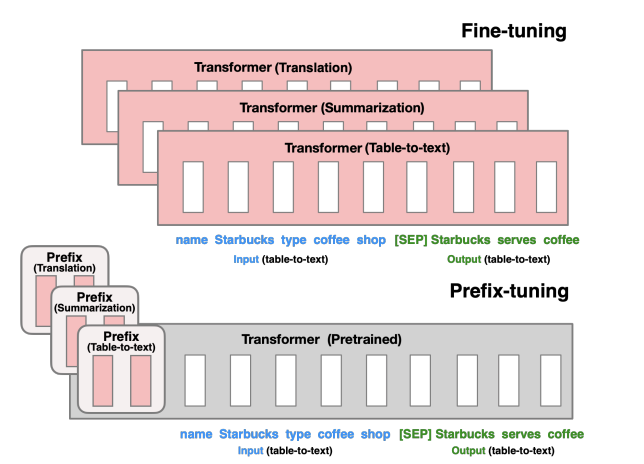
\includegraphics[width=0.8\textwidth]{chapter-2/prefix-tuning.png}
    \caption{Arsitektur \textit{Prefix-Tuning} \parencite{prefix_tuning}}
    \label{fig:prefix-tuning}
\end{figure}

Keuntungan utama dari pendekatan ini adalah efisiensi. Dengan mengoptimalkan hanya sebagian kecil dari parameter, \textit{Prefix-Tuning} dapat mencapai peningkatan kinerja dengan \textit{overhead} komputasi yang jauh lebih rendah dibandingkan dengan teknik \textit{fine-tuning} tradisional. Selain itu, dengan fokus pada \textit{prefix}, teknik ini memungkinkan adaptasi yang lebih spesifik terhadap tugas atau domain tertentu, memberikan fleksibilitas lebih dalam aplikasi praktis.

Teknik ini dapat digunakan untuk meningkatkan kinerja model generatif di berbagai tugas, termasuk penerjemahan mesin, peringkasan teks, dan lainnya. Hasil eksperimen menunjukkan bahwa \textit{Prefix-Tuning} mampu mencapai kinerja yang sebanding atau bahkan lebih baik dibandingkan dengan metode \textit{fine-tuning} tradisional, tetapi dengan biaya komputasi yang jauh lebih rendah.


% TODO : change to Bottleneck Adapter
% \subsection{\textit{Bottleneck Adapter}}

Teknik ini memperkenalkan konsep "\textit{tiny-attention}", dibandingkan dengan menambahkan lapisan adaptasi berukuran besar atau melatih ulang seluruh model. Mekanisme ini, meskipun sederhana, memungkinkan setiap posisi dalam sekuens untuk memperhatikan dan memodifikasi keadaan tersembunyinya berdasarkan informasi dari semua posisi lain dalam sekuens \parencite{tinyattention}. Dengan kata lain, setiap elemen dalam sekuens memiliki kemampuan untuk "berkomunikasi" dan "berkoordinasi" dengan elemen lain untuk membentuk representasi yang lebih kaya dan kontekstual.

Salah satu kelebihan dari pendekatan ini adalah fleksibilitas dan dinamikanya. Karena setiap posisi dapat memperhatikan semua posisi lain, model memiliki kapasitas untuk memahami hubungan antar kata dengan lebih baik, terutama hubungan yang bersifat jarak jauh atau kontekstual yang kompleks. Ini memungkinkan model untuk menangkap nuansa dan makna yang mungkin terlewatkan oleh teknik adaptasi lainnya. Arsitektur dari \textit{Bottleneck Adapter} dapat dlihat pada Gambar \ref{fig:tiny-attention}.

\begin{figure}[ht]
    \centering
    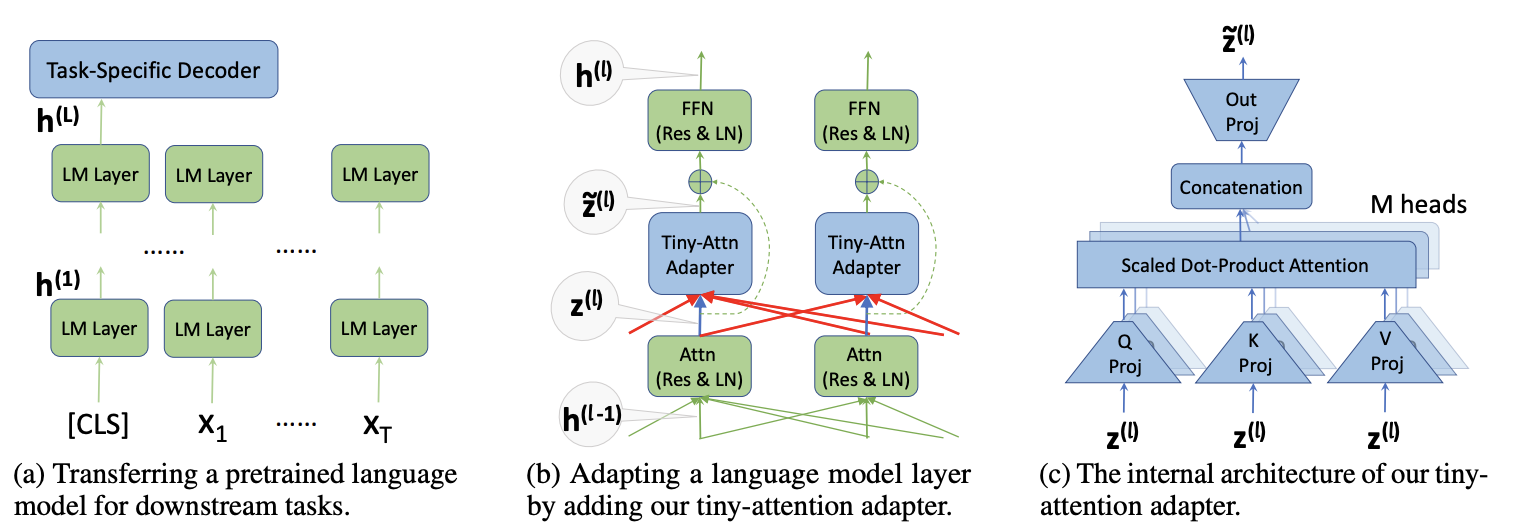
\includegraphics[width=0.8\textwidth]{chapter-2/tiny-attention.png}
    \caption{Arsitektur \textit{Bottleneck Adapter} \parencite{tinyattention}}
    \label{fig:tiny-attention}
\end{figure}


Meskipun pendekatan ini terfokus pada efisiensi parameter, \textit{Bottleneck Adapter} tidak mengorbankan kinerja. Sebaliknya, berkat mekanisme "tiny-attention", teknik ini seringkali mampu mencapai kinerja yang sebanding atau bahkan melampaui metode adaptasi tradisional, meskipun hanya dengan sebagian kecil dari parameter tambahan.


\section{Metriks Evaluasi}

Dalam proses \textit{training} model, diperlukan metode evaluasi sebagai penilaian kinerja model dengan membandingkan metriks yang dihasilkan oleh model tersebut. Metriks ini digunakan pada model klasifikasi dengan membandingkan hasil prediksi dengan target aslinya. Hasil prediksi ini dapat direpresentasikan sebagai \textit{confusion matrix}. Berdasarkan \citeauthor{metrics}, terdapat beberapa metriks yang dapat dihasilkan berdasarkan \textit{confusion matrix}, yaitu \textit{accuracy}, \textit{precision}, \textit{recall}, dan F1-\textit{Score}.

\begin{table}[ht]
\centering
\caption{\textit{Confusion matrix}}
\label{confusion-matrix}
\begin{tabular}{|l|c|c|}
\hline
\rowcolor{black!10}
\multicolumn{1}{|c|}{\textbf{Target}} & \multicolumn{2}{c|}{\textbf{Prediksi}} \\ \cline{2-3} 
\rowcolor{black!10}
& \textbf{Positif} & \textbf{Negatif} \\ \hline
\textbf{Positif} & \textit{True Positive} (TP) & \textit{False Negative} (FN) \\ \hline
\textbf{Negatif} & \textit{False Positive} (FP) & \textit{True Negative} (TN) \\ \hline
\end{tabular}
\end{table}

Berdasarkan tabel \ref{confusion-matrix} terdapat empat hasil prediksi. \textit{True Positive} (TP) yang berarti model memprediksi kelas positif yang memang bernilai positif sesuai kelasnya. True Negative (TN) memprediksi kelas negatif dan kelas tersebut memang bernilai negatif. Sedangkan, \textit{False Positive} (FP) me\textit{mprediksi kelas} positif, tetapi kelas tersebut bernilai negatif. Sebaliknya juga untuk \textit{False Negative} (FN) model memprediksi kelas tersebut sebagai negatif, tetapi kelas tersebut bernilai positif.

\subsection{\textit{Accuracy}}
Nilai \textit{accuracy} dihitung sebagai proporsi hasil prediksi yang benar (baik TP maupun TN) dari total jumlah prediksi. Metriks ini memberikan gambaran keseluruhan tentang keefektifan model. Dengan rumus sebagai berikut.

\begin{equation}
    Accuracy = \frac{TP + TN}{TP + TN + FP + FN}
\end{equation}

\subsection{\textit{Precision}}
Nilai \textit{precision} menilai proporsi prediksi positif yang benar-benar positif. Metriks ini memberikan gambaran tentang keakuratan model dalam memprediksi kelas positif. Dengan rumus sebagai berikut.
\begin{equation}
    Precision = \frac{TP}{TP + FP}
\end{equation}

\subsection{\textit{Recall}}
Nilai \textit{recall} menilai proporsi kasus positif sebenarnya yang berhasil diidentifikasi oleh model. Metrix Ini berfungsi untuk mengukur kemampuan model dalam mengidentifikasi semua kasus positif. Dengan rumus sebagai berikut.
\begin{equation}
    Recall = \frac{TP}{TP + FN}
\end{equation}

\subsection{F1-\textit{Score}}
Nilai F1-\textit{Score} direpresentasikan sebagai nilai rata-rata harmonis dari nilai \textit{precision} dan \textit{recall}. Metriks ini berfungsi untuk mengukur keseimbangan dari kedua metriks tersebut. Dengan rumus sebagai berikut.
\begin{equation}
    F1-Score = 2 \times \frac{Precision \times Recall}{Precision + Recall}
\end{equation}

\section{\textit{NLP Task Benchmarking}}

Dalam pemrosesan bahasa alami (NLP), pentingnya evaluasi kinerja model pada berbagai tugas tidak dapat diremehkan. Evaluasi memberikan cara standar untuk membandingkan berbagai model dan teknik dalam konteks aplikasi nyata.

\subsection{\textit{General Language Understanding Evaluation} (GLUE)}

GLUE, yang merupakan singkatan dari \textit{General Language Understanding Evaluation}, adalah inisiatif yang dirancang untuk memajukan pemahaman bahasa alami melalui evaluasi yang konsisten dan komprehensif \parencite{glue}. Dengan latar belakang yang semakin meningkatnya kompleksitas dan variasi model NLP, muncul kebutuhan untuk memiliki metrik evaluasi yang standar dan konsisten. 

Salah satu ciri khas dari GLUE adalah kumpulan tugas evaluasinya yang beragam. Ini mencakup tugas-tugas seperti analisis sentimen, dengan tujuannya adalah untuk menentukan apakah teks tertentu memiliki konotasi positif, negatif, atau netral; jawaban pertanyaan, dengan model diberi pertanyaan dan harus memilih jawaban yang paling tepat dari kumpulan pilihan; dan entailment teks, dengan model harus menentukan apakah satu kalimat secara logis mengikuti kalimat lain.

Namun, bukan hanya variasi tugas yang membuat GLUE menjadi penting. GLUE juga menyediakan papan peringkat, yang memungkinkan peneliti untuk membandingkan kinerja model mereka dengan model-model lain dalam kondisi yang sama. Selain itu, GLUE juga memberikan kesempatan bagi peneliti untuk memahami kelemahan dan kekuatan model mereka. Dengan memiliki berbagai tugas evaluasi, peneliti dapat melihat kelemahan dari model yang berguna untuk mengembangkan model.
\subsection{IndoLEM}
% TODO: jelasin proses eksperimen saat ini, dan datasetnya juga 
IndoLEM muncul sebagai respons terhadap kebutuhan industri dan komunitas penelitian untuk memiliki \textit{benchmark} yang khusus dirancang untuk mengevaluasi model NLP dalam konteks bahasa Indonesia \parencite{indolem}. Meskipun ada banyak \textit{benchmark} NLP yang tersedia, seperti GLUE, kebanyakan dari mereka berfokus pada bahasa Inggris. Namun, dengan keragaman linguistik yang kaya, bahasa Indonesia memerlukan pendekatan khusus dalam evaluasi model NLP.

IndoLEM tidak hanya menyediakan kumpulan tugas evaluasi yang dirancang khusus untuk bahasa Indonesia, tetapi juga memastikan bahwa tugas-tugas tersebut mencerminkan nuansa dan tantangan unik yang diasosiasikan dengan bahasa ini. Salah satu aspek penting dari IndoLEM adalah dataset yang digunakannya. Mengingat pentingnya data dalam \textit{training} dan evaluasi model NLP, IndoLEM memastikan bahwa dataset yang digunakan berasal dari sumber-sumber lokal yang relevan. Ini memastikan bahwa model yang dievaluasi dengan IndoLEM benar-benar diuji dalam konteks yang sesuai dengan penggunaan sebenarnya dalam kehidupan nyata.


% TODO: add UniPELT
\section{Penelitian Terkait}

Pada sub-bab ini, akan dibahas beberapa penelitian yang telah dilakukan terhadap penggunaan metode PETL pada \textit{pre-trained model}.
\subsection{\textit{Unified View of Parameter-Efficient Transfer Learning}}

\textit{Unified Parameter Transfer Learning} merupakan upaya untuk menggabungkan beberapa metode PETL menjadi satu kesatuan \textit{framework} \parencite{uvpl}. Dalam \textit{transfer learning}, ide utamanya adalah mengambil \textit{pre-trained model} dan menyesuaikannya untuk tugas yang berbeda. Namun, ada banyak cara untuk melakukan adaptasi ini, dan setiap metode memiliki karakteristiknya masing-masing. Beberapa teknik mungkin fokus pada penambahan lapisan adaptasi, sementara yang lain mungkin memprioritaskan modifikasi parameter tertentu dalam model.

Metode PETL lain telah berhasil mengubah atau menambahkan sedikit parameter untuk mendapatkan kinerja yang setara dengan \textit{fine-tuning} tradisional, tetapi hubungan antara metode tersebut tidak dimengerti secara baik \parencite{uvpl}. Selain itu, dicari juga elemen desain pada metode ini yang menjadi aspek penting pada kesuksesan metode terkait. \citeauthor{uvpl} pada penelitiannya ini, mencari hubungan antara tiap metode ini dengan mengupas arsitektur dari setiap metode terkait. Metode yang digunakan pada penelitian yang dilakukan oleh \citeauthor{uvpl} adalah LoRA, \textit{prefix-tuning}, dan \textit{adapter}.

\begin{figure}[ht]
    \centering
    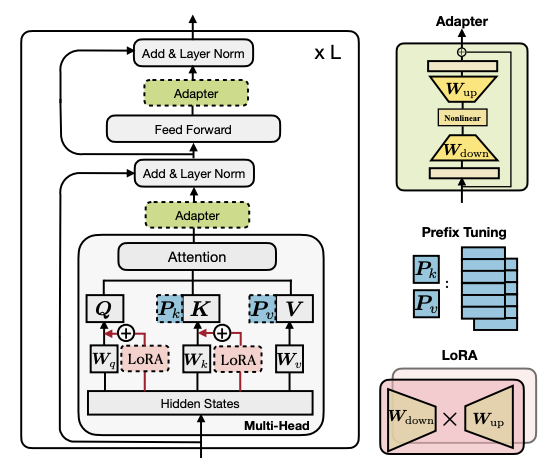
\includegraphics[width=0.8\textwidth]{chapter-2/uvpl.png}
    \caption{Arsitektur \textit{Unified View of Parameter-Efficient Transfer Learning} \parencite{uvpl}}
    \label{fig:uvpl}
\end{figure}

% TODO: tambahin secara jelas gimana tiap metode ini jadi satu dan hubungannya gimana
Arsitektur yang diajukan oleh \citeauthor{uvpl} pada penelitiannya dapat dilihat pada Gambar \ref{fig:uvpl}. Arsitektur tersebut menggabungan metode yang disebutkan sebelumnya pada model berbasis \textit{transformer}. 

\subsection{\textit{Parameter-Efficient Fine-Tuning of Large-Scale
Pre-Trained Language Models}}

Penelitian yang dilakukan oleh \citeauthor{peft_on_plm} membandingkan secara komprehensif terkait metode \textit{transfer-learning} yang efisien secara parameter pada \textit{pre-trained model}. Metode ini disebut sebagai \textit{delta-tuning} pada penelitian tersebut, dengan kata 'delta' muncul dari notasi matematika yang merepresentasikan perubahan \parencite{peft_on_plm}. Metode \textit{delta-tuning} yang digunakan adalah \textit{prompt-tuning} (PT), \textit{prefix-tuning} (PF), LoRA (LR), dan \textit{adapter} (AP). \textit{Delta-tuning} tersebut  dibandingkan dengan \textit{fine-tuning} (FT) .

Eksperimen yang dilakukan pada penelitian tersebut dilakukan pada model T5 dengan konfigurasi BASE dan LARGE. Evaluasi metode \textit{delta-tuning} pada model T5 dilakukan pada 100 tugas pemrosesan bahasa alami yang diambil dari \textit{dataset} Huggingface. Tugas yang dipilih termasuk \textit{text classification}, \textit{question answering}, dan \textit{generation}.

Berdasarkan hasil yang didapatkan pada eksperimen tersebut, metode \textit{delta-tuning} dengan pengurangan jumlah parameter yang dilatih dibandingkan dengan \textit{fine-tuning} memberikan hasil yang hampir setara pada sebagian besar tugas. Metode \textit{prefix-tuning}, LoRA, dan \textit{adapter} secara kinerja hampir mirip antara satu sama lain. Bahkan, metode \textit{delta-tuning} pada sebagian tugas mampu memberikan hasil yang dominan dibanding \textit{fine-tuning}. Secara keseluruhan, kinerja pada setiap metode dapat diurutkan sebagai berikut.

\begin{enumerate}
    \item \textit{Fine-Tuning} (FT)
    \item \textit{Low-Rank Adaptation} (LoRA)
    \item \textit{Adapter Tuning} (AP)
    \item \textit{Prefix Tuning} (PF)
    \item \textit{Prompt Tuning} (PT)
\end{enumerate}

Selain itu, dilakukan juga eksperimen terkait analisis pada efisiensi dari tiap metode. Eksperimen ini mengeksplorasi penggunaan efisiensi memori GPU pada metode \textit{delta-tuning} dan FT pada model T5 dengan konfigurasi BASE, LARGE, dan XL. Metode \textit{delta-tuning} yang digunakan adalah LoRA (LR), dan \textit{adapter} (AP), dan BitFit (BF). Berdasarkan Gambar \ref{fig:peft_on_plm_memory}, penggunaan memori pada setiap metode \textit{delta-tuning} berkurang dibandingkan dengan \textit{fine-tuning}. Hasil ini menunjukkan bahwa \textit{delta-tuning} mengurangi penggunaan memori GPU dengan mengurangi kebutuhan komputasi gradien untuk mengubah parameter.

\begin{figure}[ht]
    \centering
    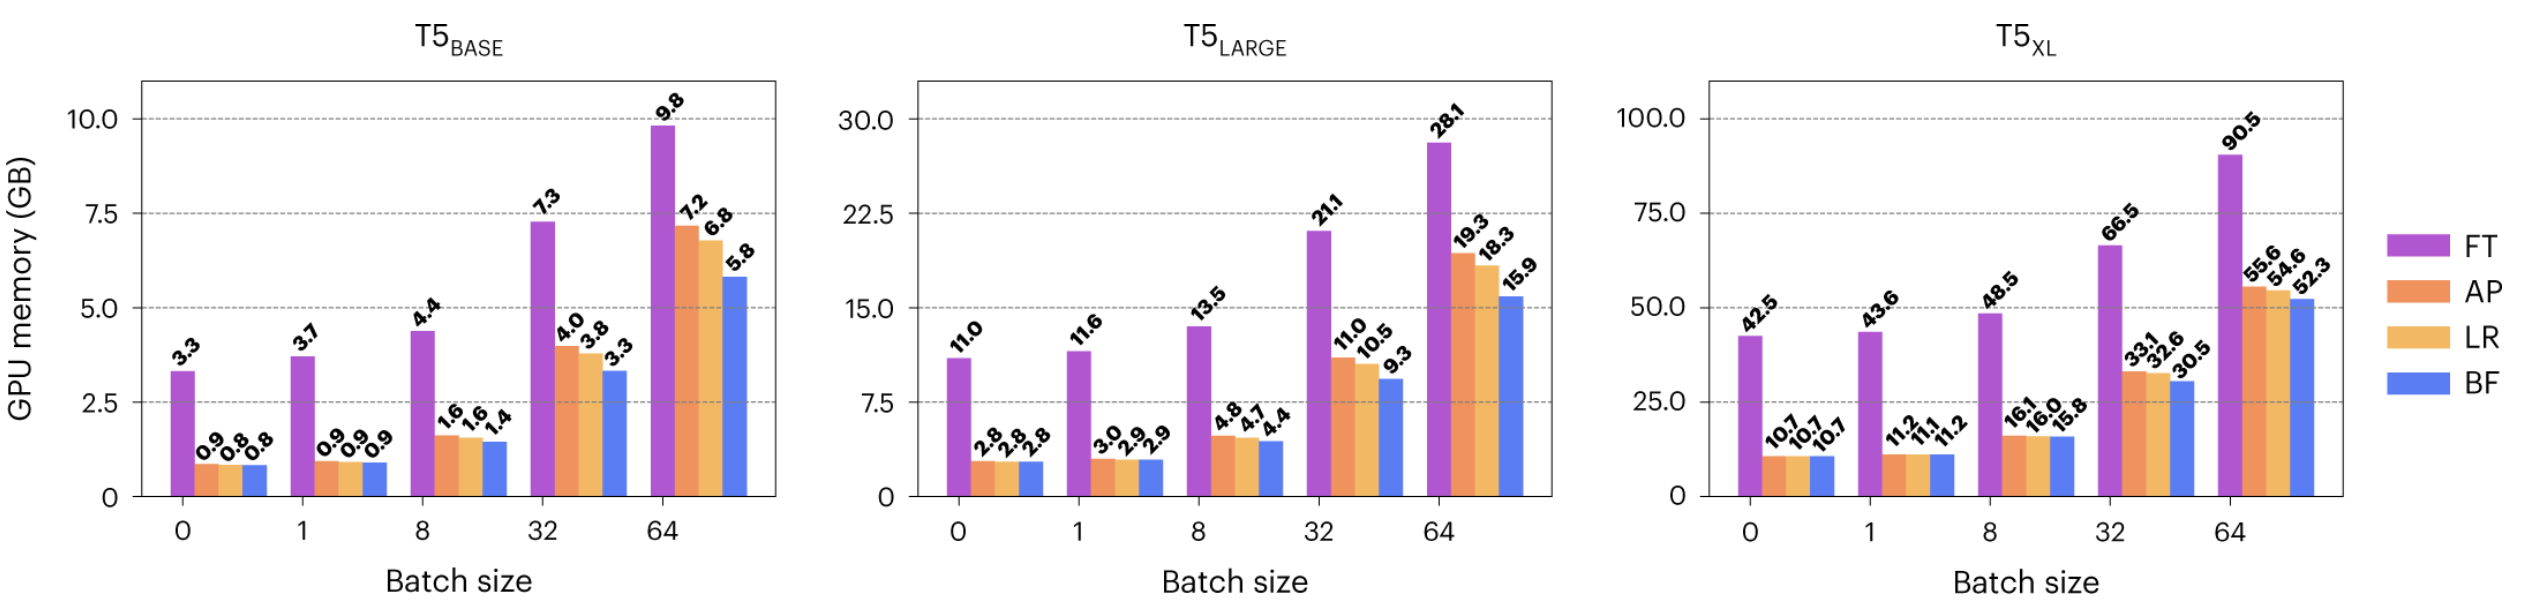
\includegraphics[width=1\textwidth]{chapter-2/peft_on_plm_memory.png}
    \caption{Perbandingan Efisiensi Memori \parencite{peft_on_plm}}
    \label{fig:peft_on_plm_memory}
\end{figure}

